\documentclass[assd_tp2_main.tex]{subfiles}

\begin{document}

\section{Síntesis de sonidos mediante modelos f\'isicos}
Se analizarán dos variantes del modelo Karplus-Strong en paralelo, tanto de manera teórica como práctica. 

\subsection{Bloque A Elemental}
Se resolverá, como cálculo auxiliar un bloque sencillo definido como:
\begin{figure}[H]	
	\centering
	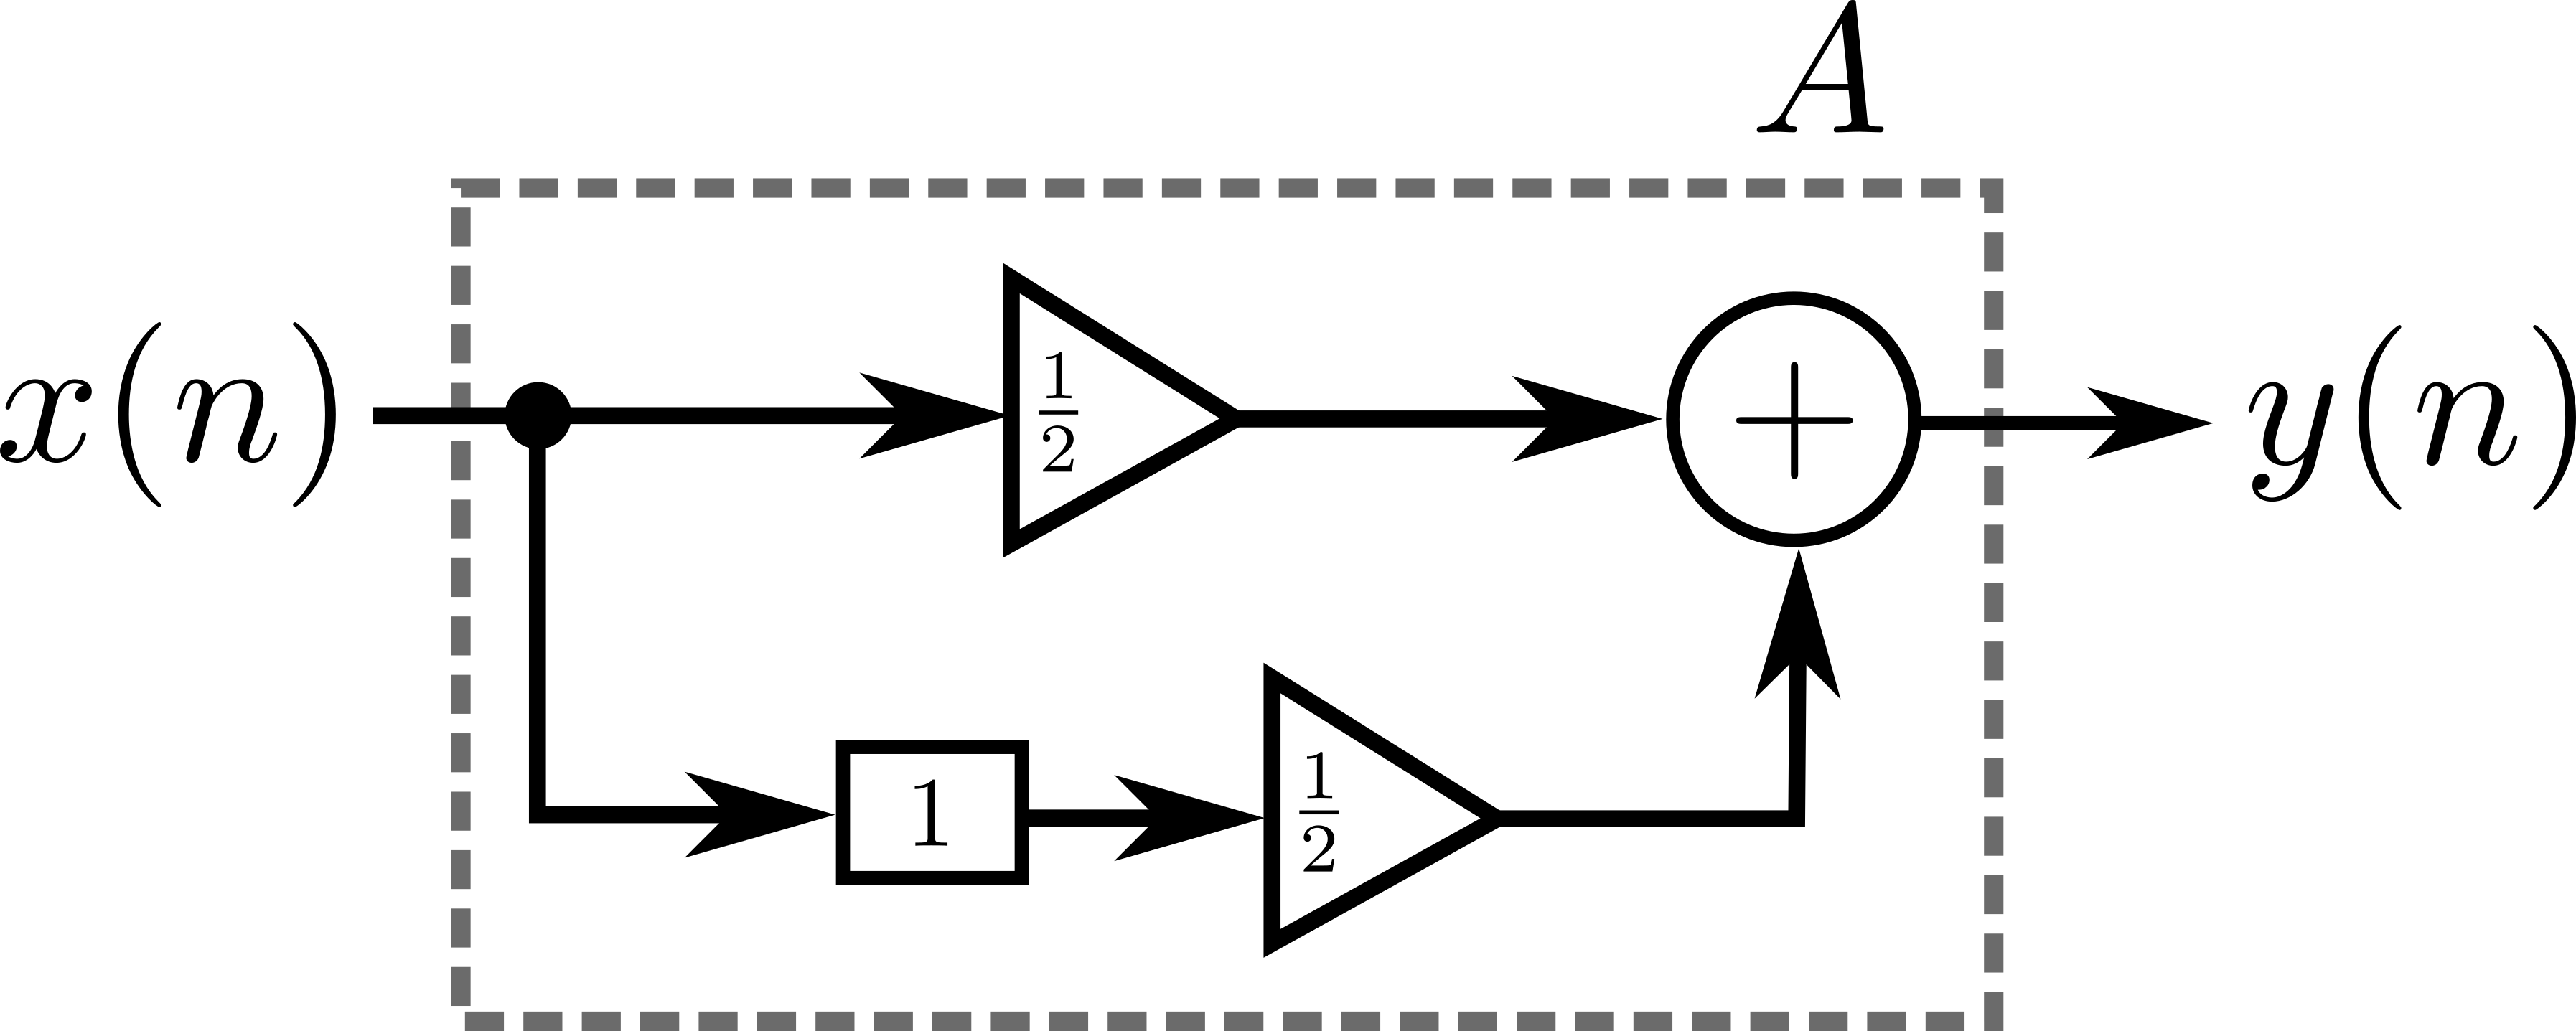
\includegraphics[scale=1]{graficos/bloque1ej5.png}
	\caption{Bloque elemental}
	\label{fig:bloqueElemental}
\end{figure}

Este bloque solo promedia los dos ultimos valores de entrada. Su transferencia esta dada por
\begin{equation}
x(n)=\frac{1}{2}x(n)+\frac{1}{2}x(n-1)
\end{equation}
\begin{equation}
Y(z)=\frac{1}{2}X(z)+\frac{1}{2}X(z)z^{-1} \implies A(z)=\frac{z+1}{z}
\end{equation}
Se puede observar que el bloque A es pasa-bajos (cero en $Z=-1$); lo cual es, en principio, razonable, el bloque A suaviza la entrada.

\subsection{Karplus Strong 1}
\subsubsection{Análisis teórico}
Se resolverá un nuevo sistema, denominado $S_1$, el cuál consiste en una adicion de realimentación al sistema anterior.
\begin{figure}[H]	
	\centering
	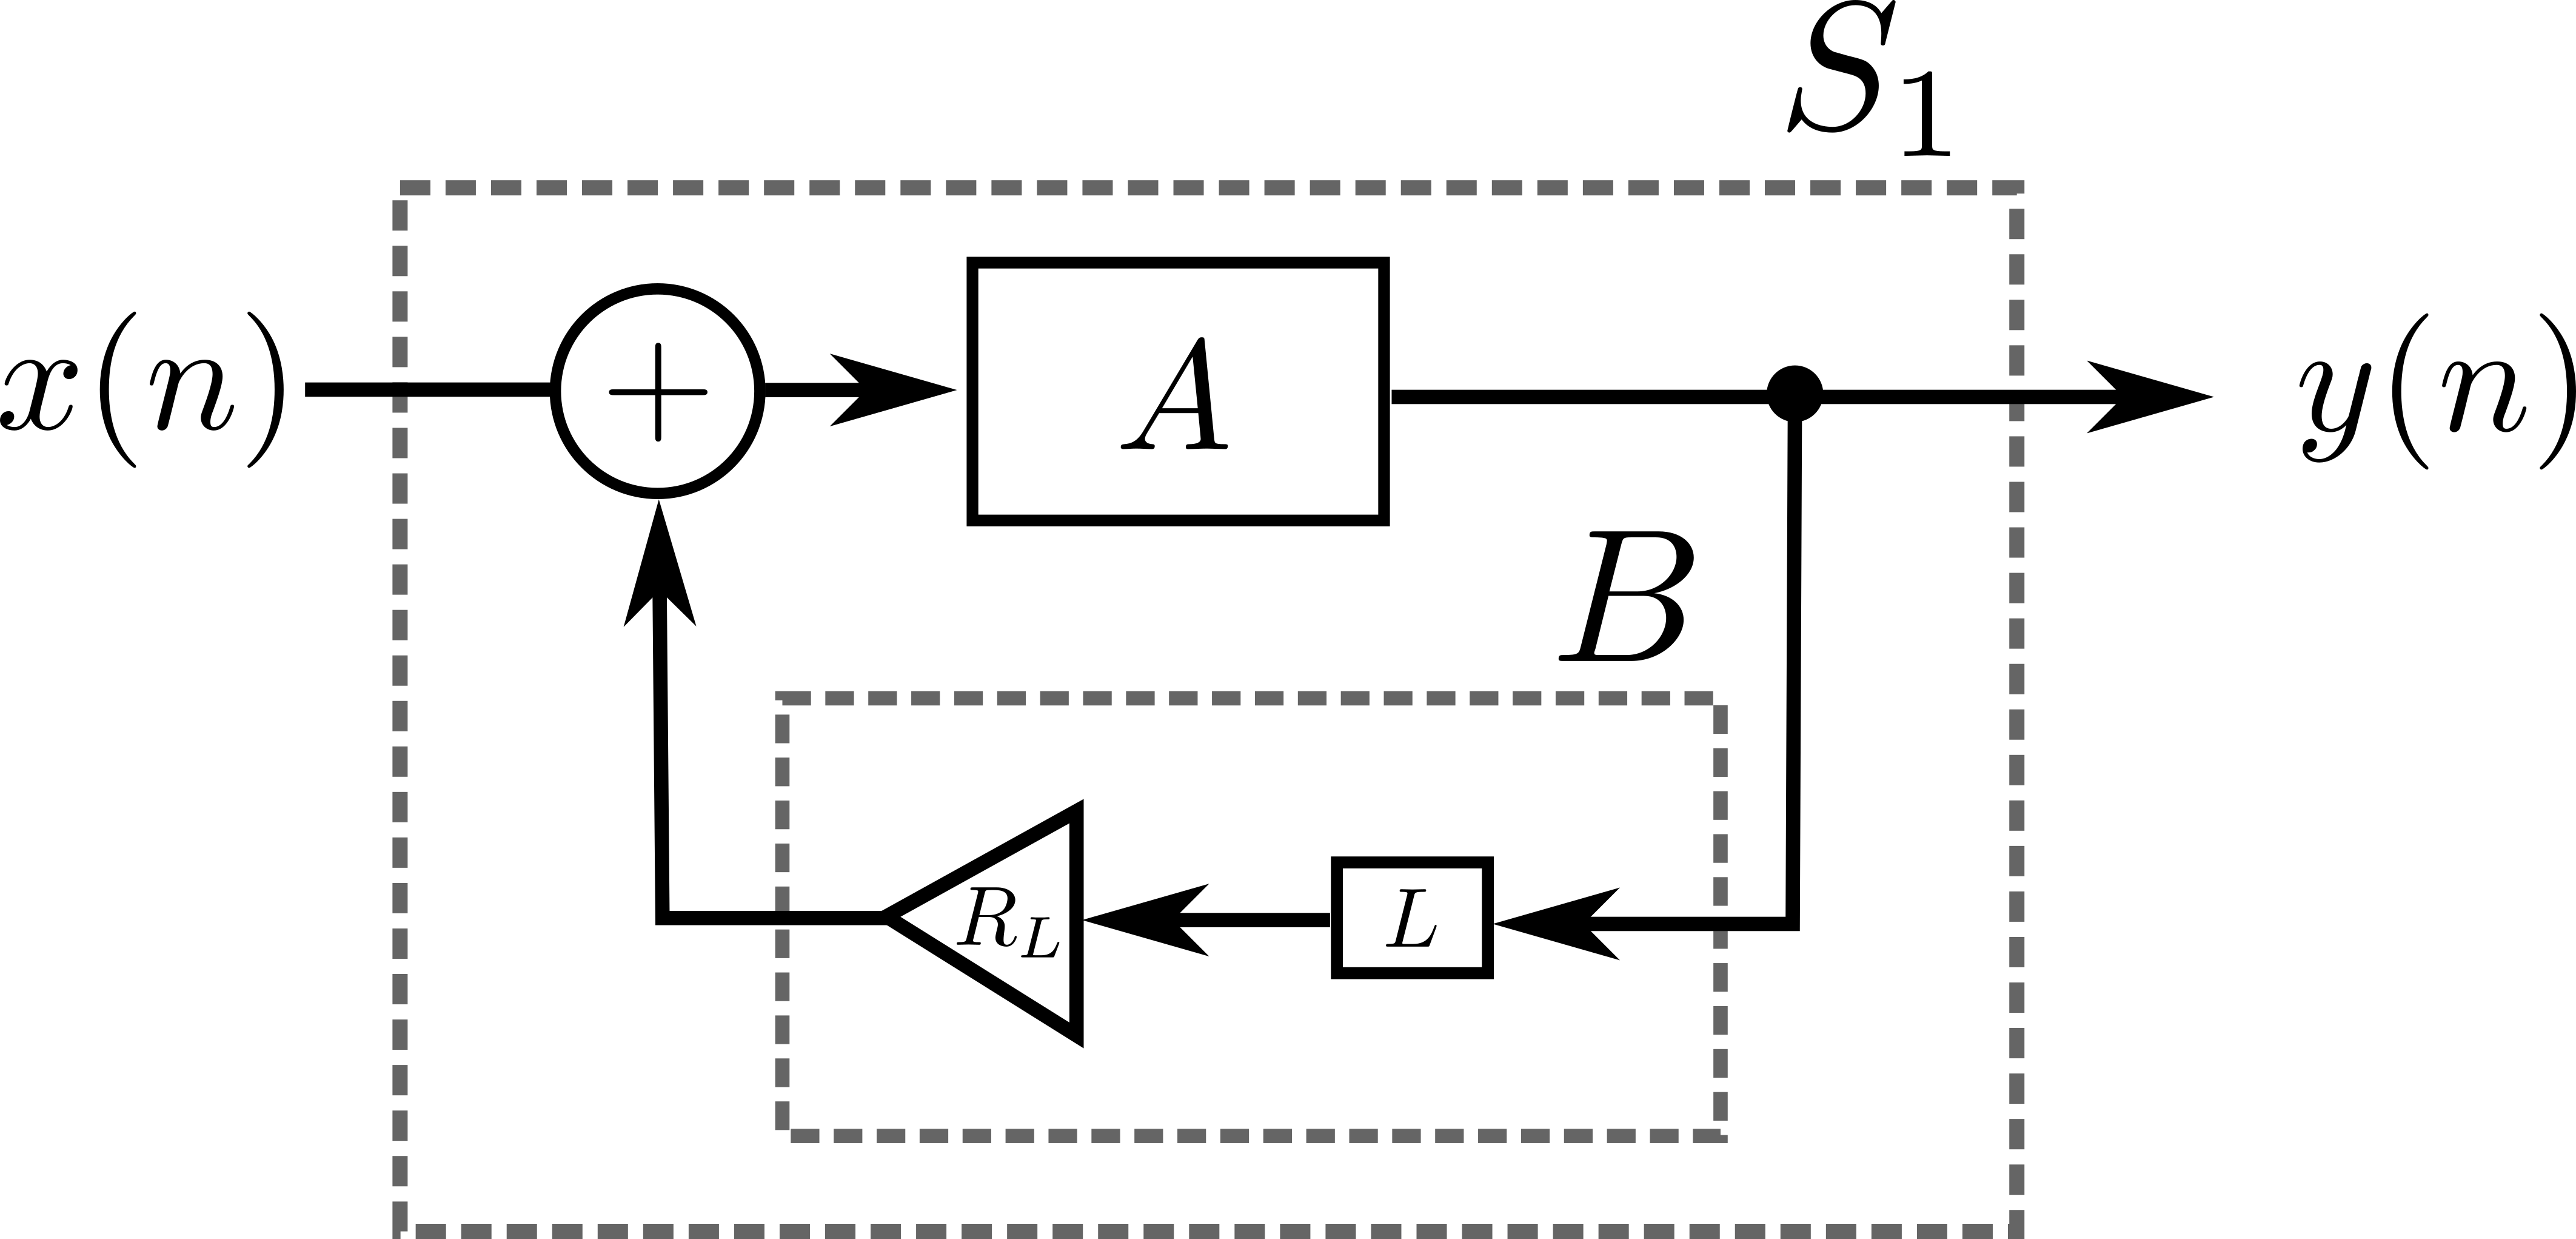
\includegraphics[scale=1]{graficos/bloque2ej5.png}
	\caption{Bloque elemental}
	\label{fig:bloqueElemental}
\end{figure}

Mediante teoria de feedback a considerando que $B(z)=z^{-L}R_L$ se llega a que
\begin{equation}
S_1(z)=\frac{\frac{1}{2}+\frac{1}{2}z^{-1}}{1-\frac{1}{2}R_Lz^{-L}-\frac{1}{2}R_Lz^{-L-1}}=\frac{ \frac{1}{2} z^{L+1} + \frac{1}{2}z^L}{ z^{L+1} - \frac{1}{2}R_L z-\frac{1}{2}R_L } 
\end{equation}
\begin{equation}
y(n)=\frac{1}{2}x(n)+\frac{1}{2}x(n-1)+\frac{1}{2}R_Ly(n-L)+\frac{1}{2}R_Ly(n-L-1)
\end{equation}

Es decir, una expresión con $L+1$ polos y $L+1$ ceros, en otras palabras, una ecuación diferencial de orden $L+1$ con vector de longitud $L$ como condición inicial. De la ecuación de diferencias se puede observar que la unica forma de garantizar estrictamente la estabilidad del sistema será exigiendo $R_L<1$. No obstante, en la práctica como la frecuencia de resonancia del sistema no será exacta; colocar $R_L=1$ no provocará inestabilidad. Más aun; resulta provechoso aproximar $R_L$ a $1$ lo más posible para lograr estirar la duración de las oscilaciones.   

\subsubsection{Estudio de la distribución polos y ceros, respuesta en frecuencia}
\begin{figure}[H]	
	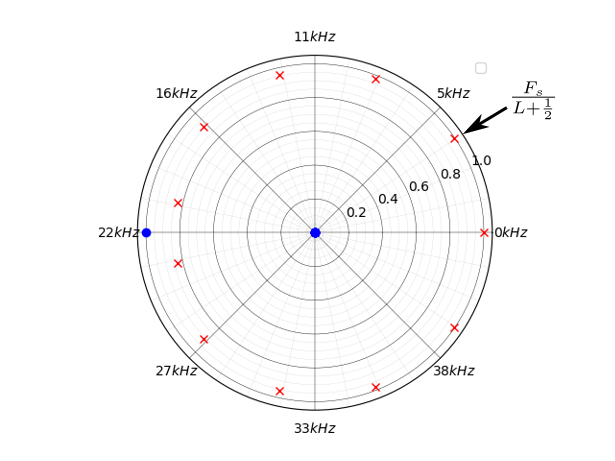
\includegraphics[scale=0.45]{graficos/polos.png}
	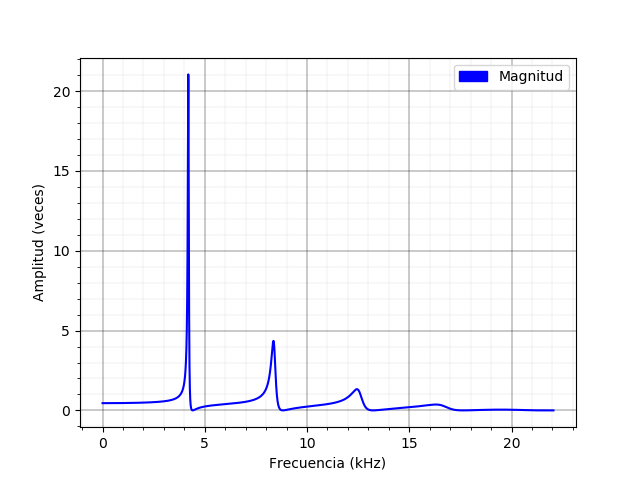
\includegraphics[scale=0.58]{graficos/freq_response.png}
	\caption{Polos y ceros (derecha), Rta en frecuencia (izquierda), $S_1$ con $R_L=1$, $L=10$, $f_s=44.1kHz$}
	\label{fig:polosCeros}
\end{figure}

Del diagrama de polos y ceros y la respuesta en frecuencia podemos observar que hay una frecuencia de resonancia $F_R=F_s/(L+\frac{1}{2})$ que tiende a cumplir las hipotesis del criterio de Barkhausen, y por lo tanto provocar oscilaciones, lo cuál es el objetivo del bloque; conseguir una salida que perdure en el tiempo a partir de una entrada de longitud $L$ muy corta.

\subsubsection{Cálculo de $F_R$}
Se mostrará porque el sistema resuena en $F_R=F_s/(L+\frac{1}{2})$. En la sección anterior se observó que la frecuencia de resonancia debía ser aquella que tendiera a cumlir las hipotesis del criterio de barkhausen; en otras palabras; que la ganancia del lazo se aproxime a $1$ con $0$ grados. 
El sistema esta compuesto por la superposición de un sistema con un retraso de lazo $L$ y otro sistema con retraso de lazo $L+1$. Por lo tanto; para que una señal no tienda a interferirse al recorrer el lazo debe tener periodo $\frac{L+L+1}{2}$; es decir una frecuencia $\frac{F_s}{L+1/2}$

\subsubsection{Análisis mediante señales}
 
Se procederá a estudiar como el sistema responde a diversas entradas, entre ellas, un impulso unitario, ruido gaussiano de longitud $L$, y ruido lineal de longitud $L$. Se decidió aumentar $L$ en estos casos a $50$ para conseguir frecuencias más cercanas a las audibles.
 
\begin{figure}[H]
	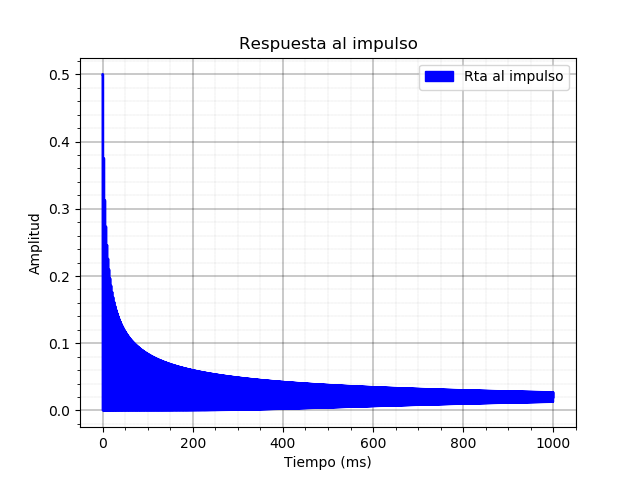
\includegraphics[scale=0.55]{graficos/impulsoBloqueS1.png}
	\includegraphics[scale=0.41]{graficos/impulsoBloqueS1Zoom.png}
	\caption{Respuesta al impulso con y sin zoom, $R_L=1$, $L=50$, $f_s=44.1kHz$}
\end{figure}

Se puede observar que, de todas las frecuencias pertenecientes al impulso, la más amplificada vale $865Hz \approx \frac{F_s}{1/2+L}$. Por otro lado es importante observar que la salida se encuentra montada sobre una tensión continua, más precisamente, nunca es menor que 0. Esto se debe a que cuando la excitación es exclusivamente positiva, como la realimentación es positiva y no hay inversiones la salida siempre será positiva. Por ello es importante que la excitación inicial sea tanto positiva como negativa para lograr que la salida este centrada en 0.

\begin{figure}[H]
	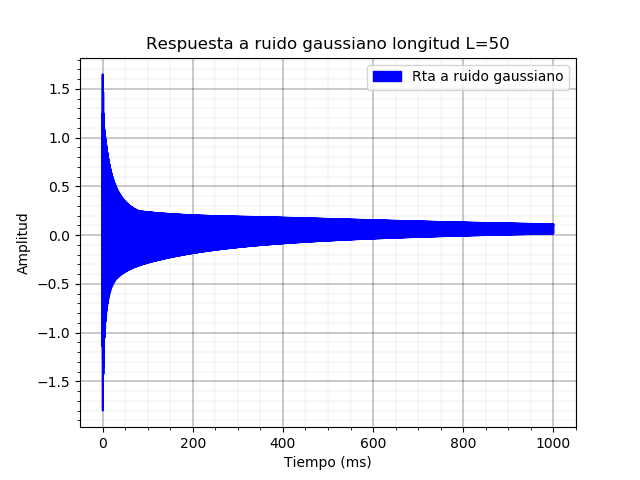
\includegraphics[scale=0.55]{graficos/gaussBloqueS1.png}
	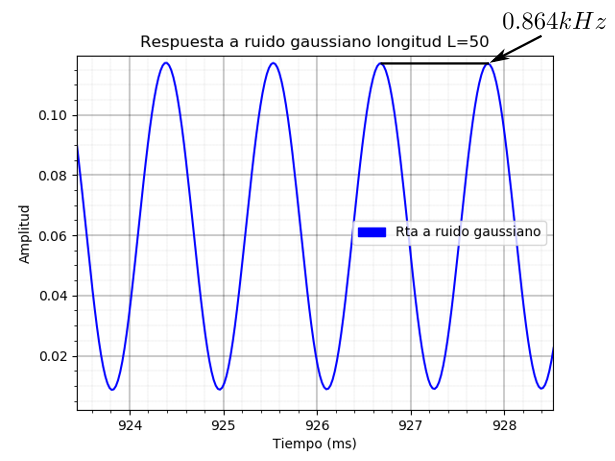
\includegraphics[scale=0.41]{graficos/gaussBloqueS1zoom.png}
	\caption{Respuesta a entrada Gaussiana con y sin zoom, $R_L=1$, $L=50$, $f_s=44.1kHz$}
\end{figure}

Se puede ver que la salida fue a la misma frecuencia que en el caso anterior, al mismo tiempo que nuevamente, estuvo montada sobre una continua. No obstante la salida tuvo la posiblidad de tomar valores negativos.

\begin{figure}[H]
	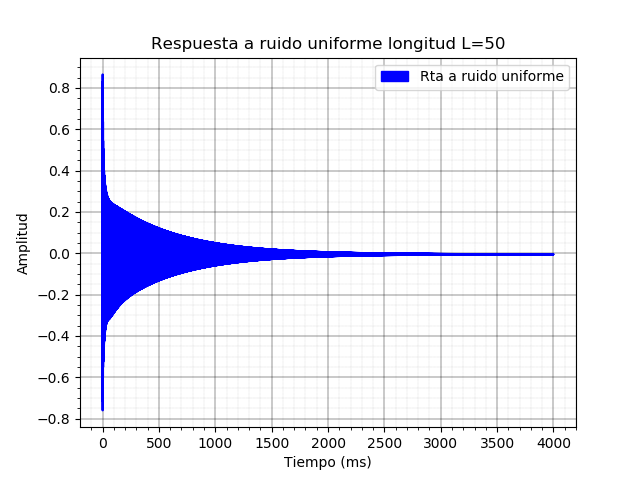
\includegraphics[scale=0.55]{graficos/randomBloqueS1.png}
	\includegraphics[scale=0.55]{graficos/randomBloqueS1zoom.png}
	\caption{Respuesta a entrada de ruido uniforme con y sin zoom, $R_L=1$, $L=50$, $f_s=44.1kHz$}
\end{figure}

Podemos observar que la salida fue similar a la de ruido gaussiano

\subsection{Karplus Strong 2}

\subsubsection{Analisis teórico elemental}
Se estudiará un nuevo sistema con una pequeña modificación la cual consiste en agregar un multiplicador en el bloque realimentador, cuyo valor es aleatorio, puede ser 1 o -1. La probabilidad de que sea 1 se llamará $b$ 
\begin{figure}[H]
	\begin{center}
	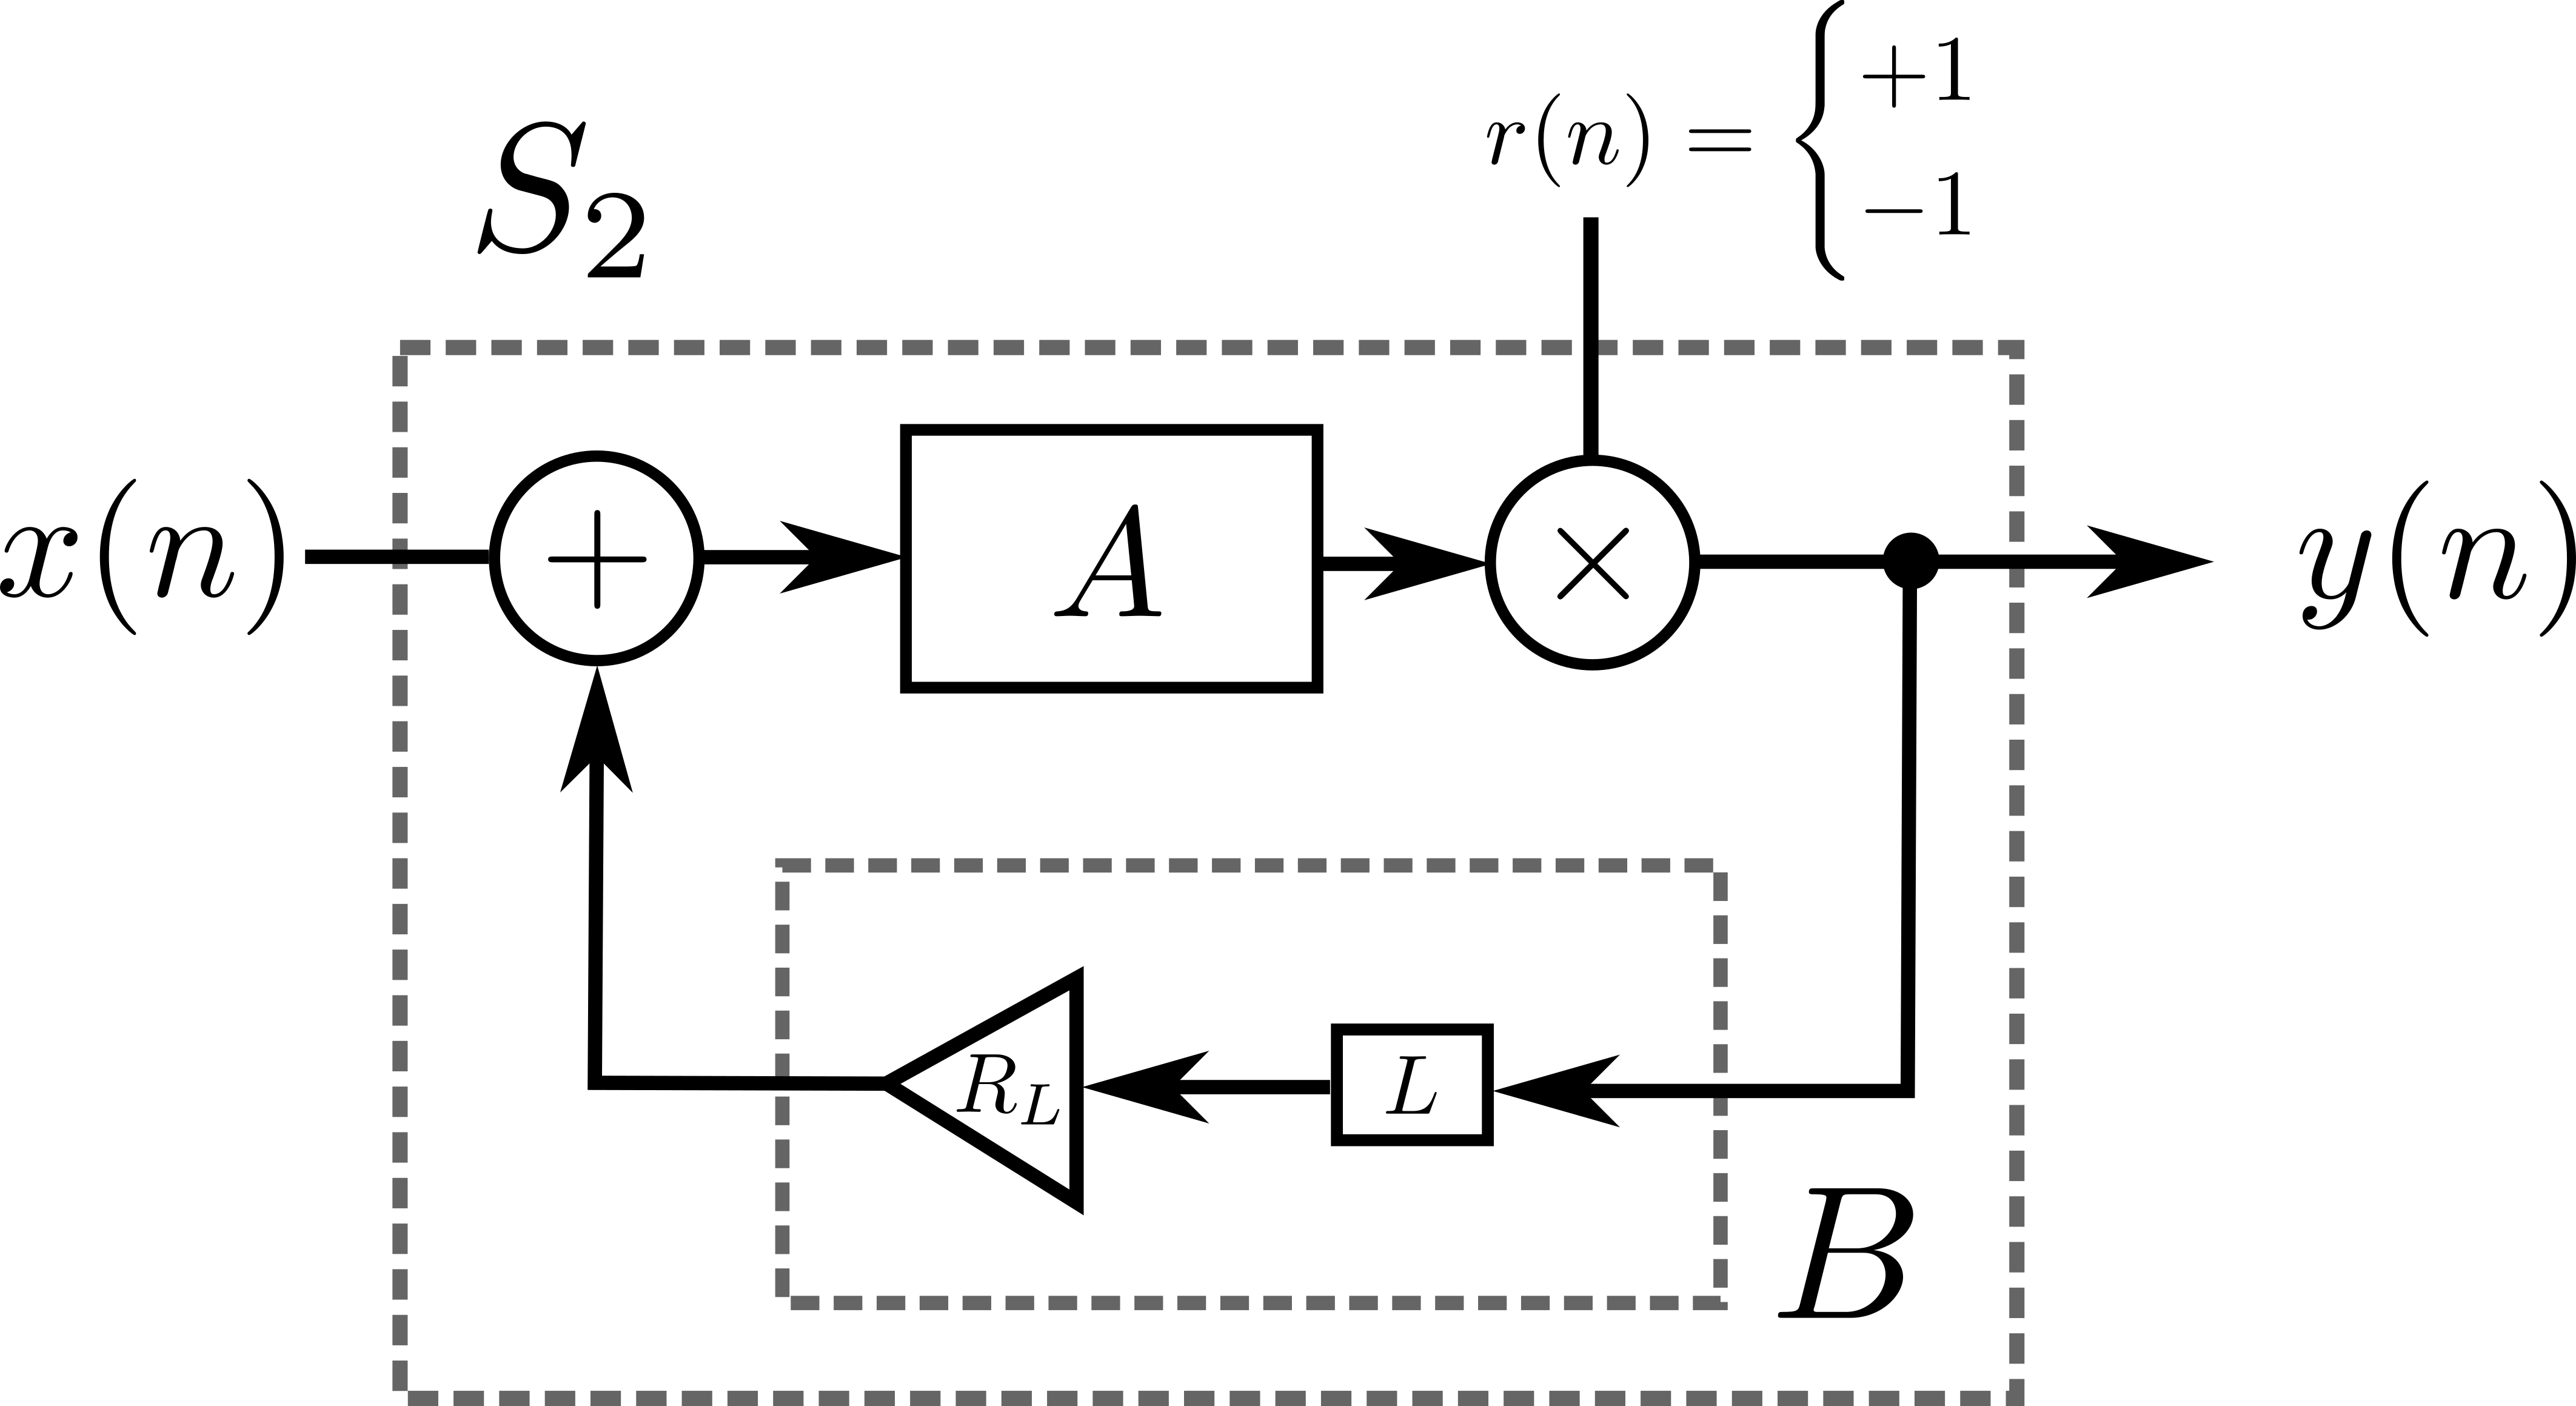
\includegraphics[scale=1]{graficos/bloque3ej5.png}
	\caption{Diagrama del sistema $S_2$}

	\end{center}
\end{figure}

Escrito en lenguaje matemático

\begin{equation}
	A(z)=b(\frac{1}{2}+\frac{1}{2}z^{-1})
\end{equation}
\begin{equation}
	B(z)=\frac{1}{2}z^{-L}
\end{equation}

Usando teória de feedback concluimos que

\begin{equation}
	S_2(z)=\frac{\frac{1}{2}r+\frac{1}{2}rz^{-1}}{1-\frac{1}{2}rR_Lz^{-L}-r\frac{1}{2}R_Lz^{-L-1}}
\end{equation}
\begin{equation}
	y(n) = \frac{1}{2}rx(n) + \frac{1}{2}rx(n-1) + \frac{1}{2}rR_Ly(n-L)+\frac{1}{2}rR_Ly(n-L-1)
\end{equation}
Observamos de la ecuación de diferencias que el sistema es prácticamente equivalente al anterior con una diferencia; ahora la salida se invierte de manera aleatoria ciclo a ciclo. Esta aleatoriedad ayudará a simular la aleatoriedad de un sonido percutido.
\subsubsection{Respuesta en frecuencia}

Debido a la complejidad trigonometricá del cálculo exacto se opto por aproximar númericamente el gráfico de $\phi(w)=\angle H(e^{jw})$ (respuesta en frecuencia del sistema) 
Por otro lado se decidió tampoco realizar el cálculo de la frecuencia de resonancia con exactitud, debido a su elevada complejidad. En realidad no es estrictamente necesario, en realidad en la práctica cuando $b$ sea distinto de 1 o 0 ocurrira notable interferencia en el lazo que destruira la resonancia; lo cual provocará que el sonido se extinga luego de breves instantes.

Ahora se mostrará la respuesta en frecuencia con $b=1, b=\frac{1}{2}, b=0$. Es importante observar que dado que la salida es estrictamente una variable aleatoria, la respuesta en frecuencia entonces estrictamente también es una variable aleatoria. Se decidió mostrar el valor medio de dicha variable aleatoria.

\begin{figure}[H]
	\begin{center}
	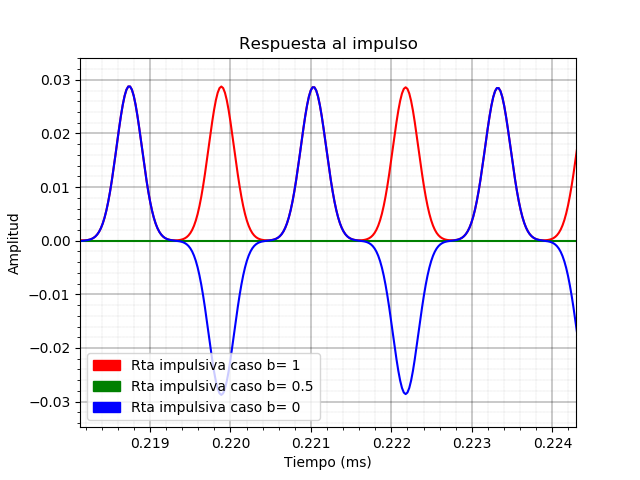
\includegraphics[scale=0.5]{graficos/impulsoB.png}
	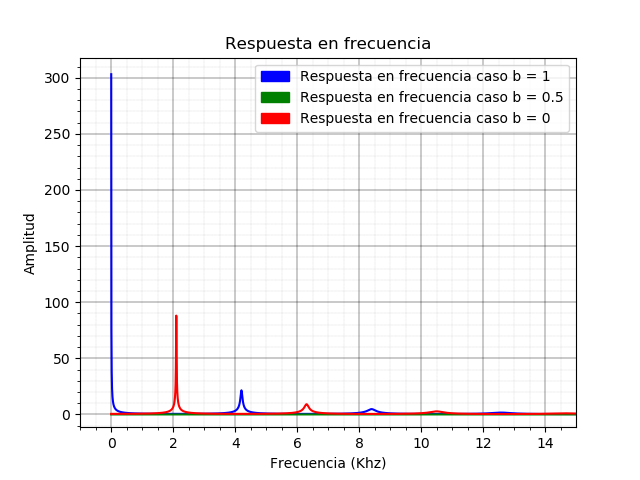
\includegraphics[scale=0.5]{graficos/rtaFreqB.png}
	\caption{Respuesta al impulso y en frecuencia con $b=1, 0.5, 0$ (izquierda a derecha)}

	\end{center}
\end{figure}

Se observa que, como fue predicho, en el caso b=0.5 todas las frecuencias son destruidas luego de un pequeño transitorio. Además, se observó que el caso de b=0 mostró una inversión espectral que provocó que la frecuencia de resonancia se redujerá en dicho casó lo cual implicó un sonido más grave, como el de un arpa.
También se observó una gran amplificación en el caso $b=1$ en la continua. Esto no es un gran problema ya que si la entrada tiene valor medio cercano a 0 y se filtra dicha componente a la salida es un problema evitable.


\section{Sintetización de instrumentos}

En base a las distintas pruebas realizadas anteriormente se procederá a realizar las funciones que permitan sintetizar el sonido de varios instrumentos que son:
\begin{itemize}
	\item Arpa
	\item Guitarra
	\item Tambor (percusión)
\end{itemize}

\subsection{¿Como tener libertad con la frecuencia fundamental?}

La primera necesidad fue tener la libertad de poder sintetizar un sonido con cualquier frecuencia que se necesite. La solución fue sencilla; consistió en modificar el bloque $A$ para que nos permita una mayor libertad al elegir la frecuencia
\begin{figure}[H]
	\begin{center}
	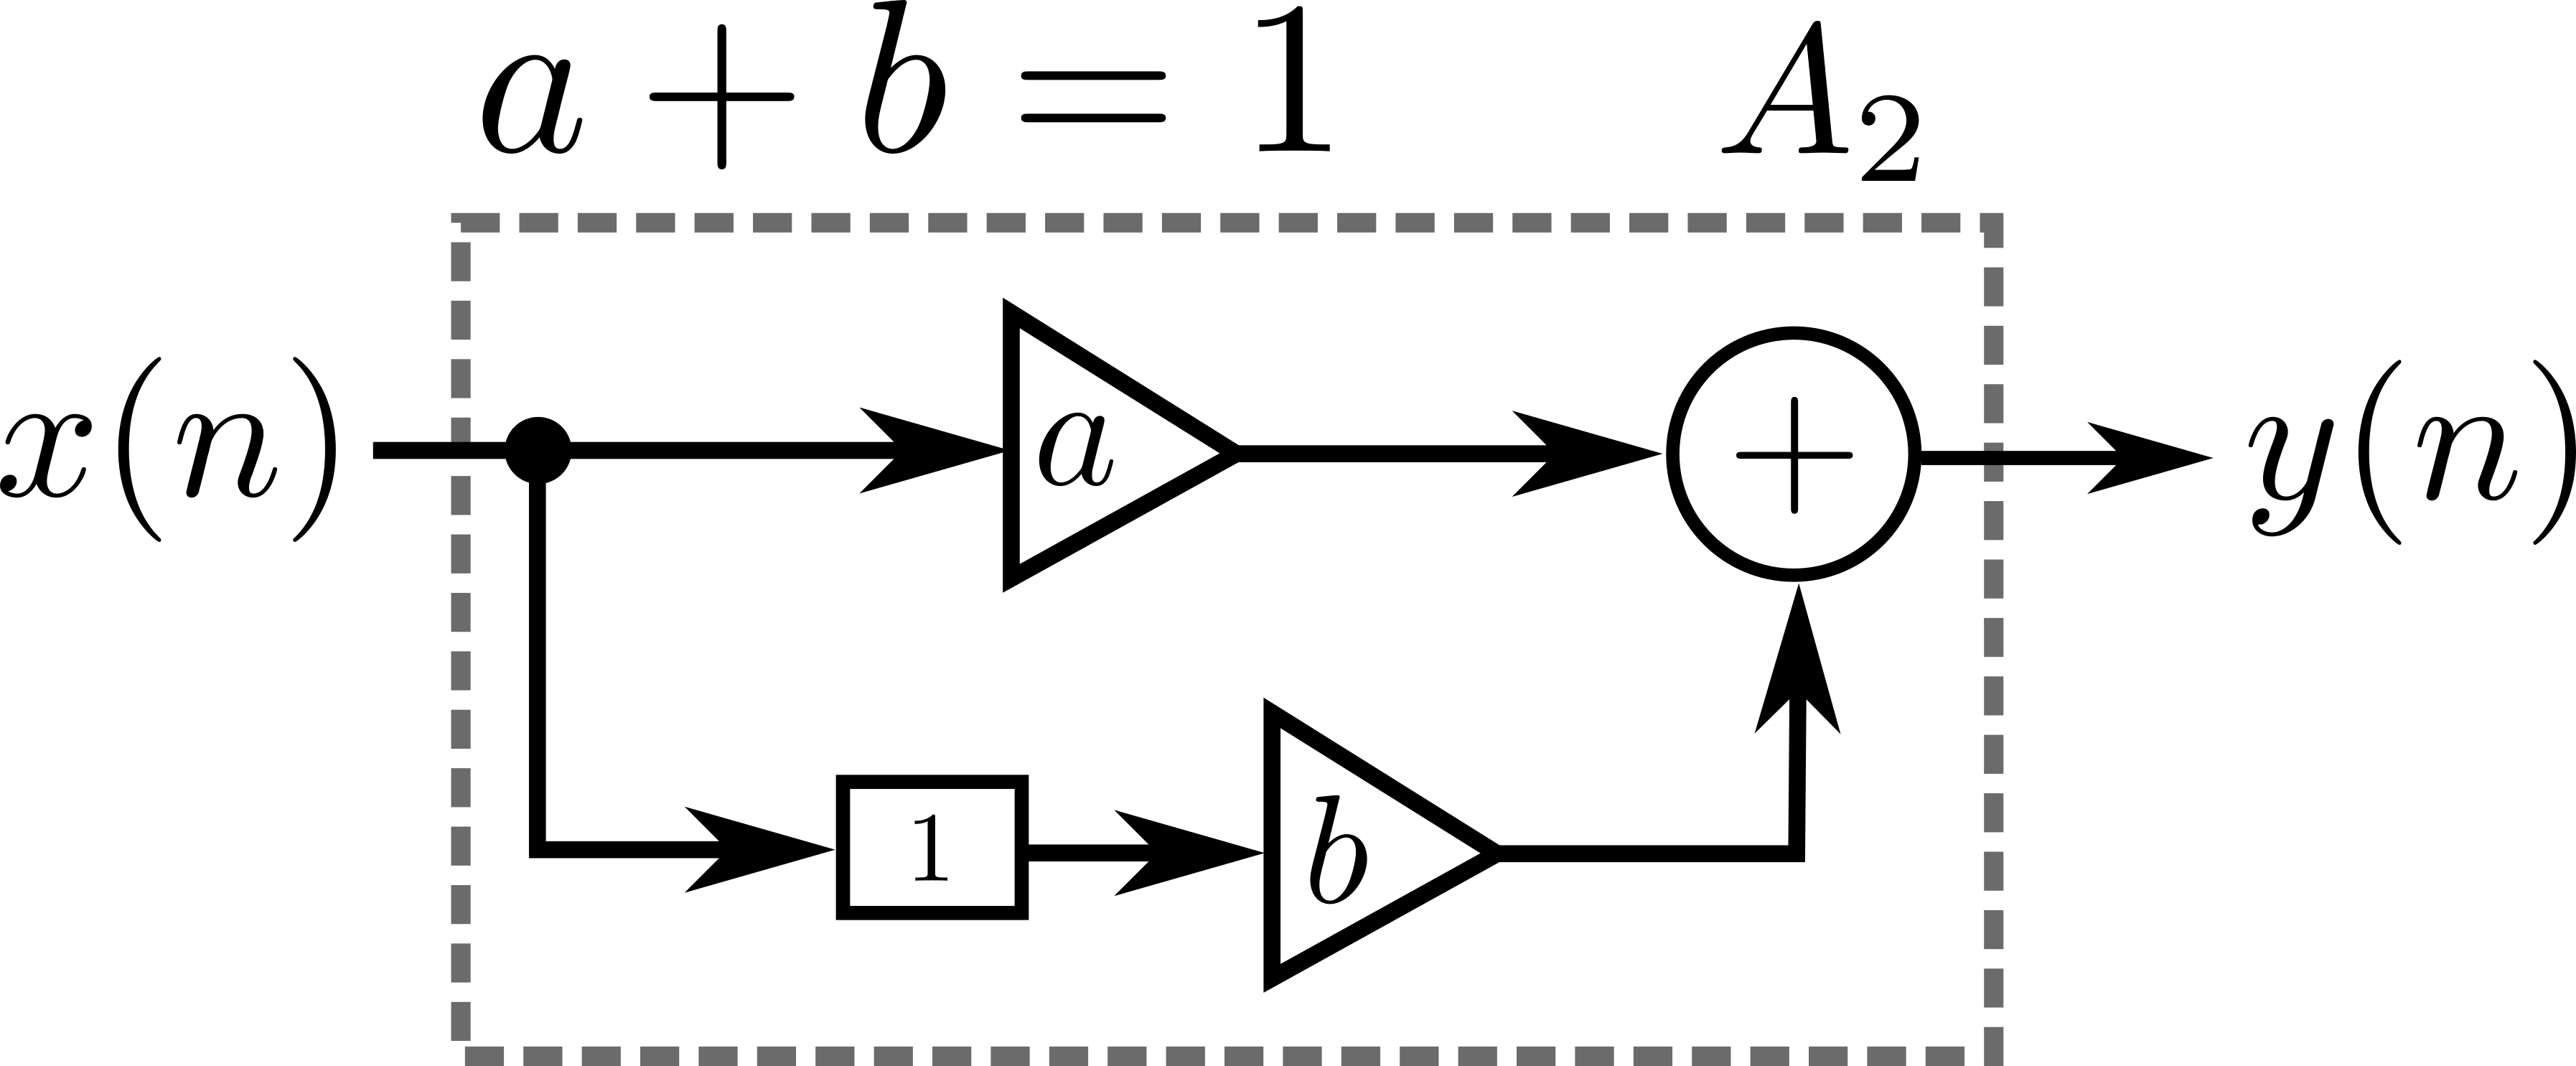
\includegraphics[scale=1]{graficos/bloque4ej5.png}
	\caption{Modificación bloque $A$ para poder personalizar la frecuencia}

	\end{center}
\end{figure}

Con la nueva modificación la frecuencia de resonancia paso a estar dada por

\begin{equation}
	F_R=F_s(a\frac{L}{2}+b\frac{L+1}{2})
\end{equation}

Eligiendo $L$ adecuadamente se puede garantizar que existan $a$ y $b$ entre 0 y 1 que verifiquen la ecuación anterior

\subsection{¿Comó filtrar la componente continua?}
Se colocó un filtro pasabajo al final del filtro para elimiar la ``molesta'' componente continua que el sistema poseeía. Dicha característica de la señal era aleatoria e impredecible por lo tanto fue muy importante colocar dicho filtro.

\subsection{¿Como atenuar el sonido de manera suave?}
Cuando termina el sonido la amplitud no puede ser disminuida de manera inmediata. Se necesito entonces multiplicar la señal por una ventana para regular la duración y provocar una disminución gradual de la intensidad del sonido

\begin{figure}[H]
	\begin{center}
	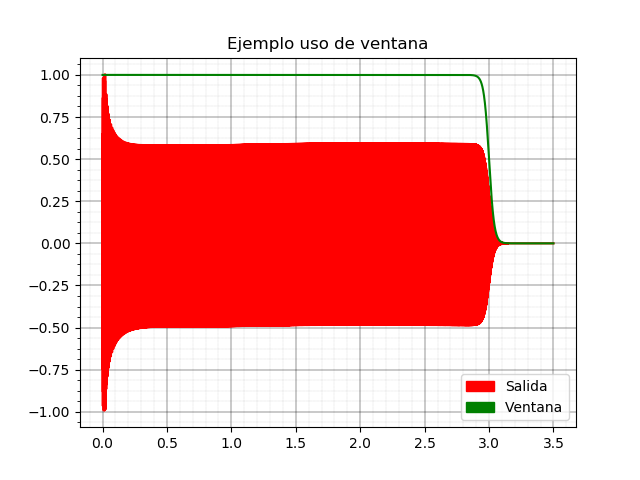
\includegraphics[scale=0.5]{graficos/ejemplo_uso_ventana.png}
	\caption{Ejemplo uso de ventana}

	\end{center}
\end{figure}
Los resultados del uso de ventanas fueron satisfactorios, la atenuación del sonido se observó de forma gradual

\subsection{Sintetización de sonido de guitarra}
Se implemento el sonido de una guitarra utilizando el modelo Karplus Strong utilizando la modificación que permitió una elección continua de frecuencias. A continuación se mostrará el espectograma del sonido de la guitarra producido.

\begin{figure}[H]
	\begin{center}
	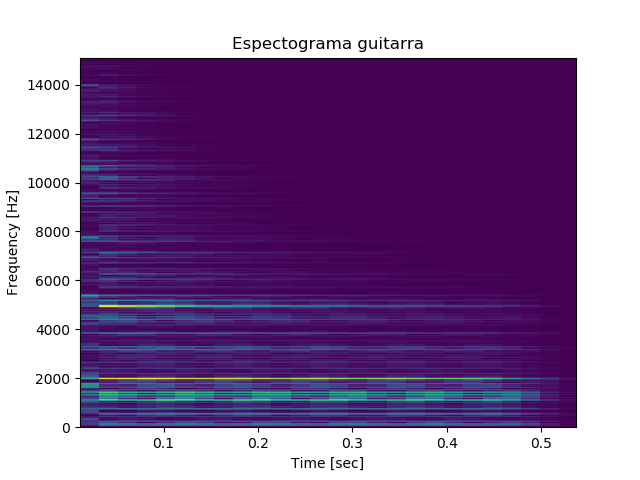
\includegraphics[scale=0.5]{graficos/espectograma_guitarra.png}
	\caption{Espectograma sonido de guitarra generado, nota: $A_0=440 Hz$}

	\end{center}
\end{figure}
El sonido escuchado fue como el de una guitarra, por lo tanto se consider\'o que los resultados fueron satisfactorios; los armónicos se aproximaron a los de una guitarra acústica.


\subsection{Distorsión del sonido de guitarra}
Se distorsionó el sonido de una guitarra utilizando una modificación al modelo. Se colocó un valor de $R_L>1$ pero, utilizando una funcion normalizadora (entre -1 y 1) se conformó un control automatico de ganancia que evitó la inestabilidad del sistema. Colocando diversos valores de $R_L$ se armó distorsión de distintos tipos. 
Se mostrará un espectograma de uno de los sonidos generados

\begin{figure}[H]
	\begin{center}
	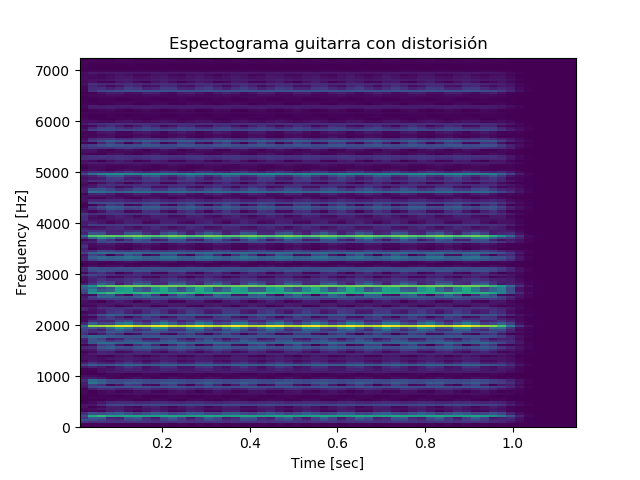
\includegraphics[scale=0.5]{graficos/espectograma_guitarra_distorsion.png}
	\caption{Espectograma sonido de guitarra con distorsión, $R_L=2$, nota: $A_0=440 Hz$}

	\end{center}
\end{figure}
Se observa que en general los armónicos generados producto de la distorsión son muchos más numerosos y además tienden a tener una frecuencia mayor que los de la guitarra acústica. 
El sonido generado fue percibido como el de un sonido eléctrico, que sonaba bien pero que no se asocia a ningún instrumento acústico.
 
\subsection{Sintetización de instrumento de percusión}

Utilizando la modificación del modelo de Karplus Strong la cual establec\'ia una variable aleatoria se sintetiz\'o el sonido de instrumentos de percusión. Se necesit\'o aplicar algunas modificaciones, en primer lugar se decidió colocar un valor de $L$ elevado para elevar el tiempo de decaimiento. Por otro lado, se provocó que el est\'imulo al sistema cayera de manera abrupta, de otra manera no se podía observar el sonido percutido, sino simplemente ruido. A continuación se mostrará la salida en el tiempo y en frecuencia.

\begin{figure}[H]
	\begin{center}
	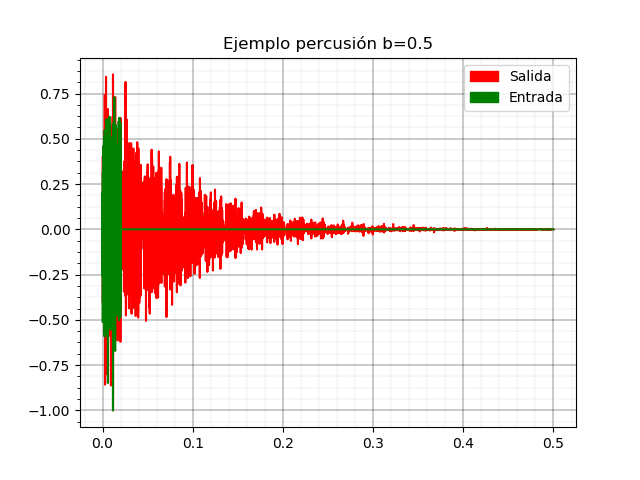
\includegraphics[scale=0.5]{graficos/ejemplo_percusion_tiempo.png}
	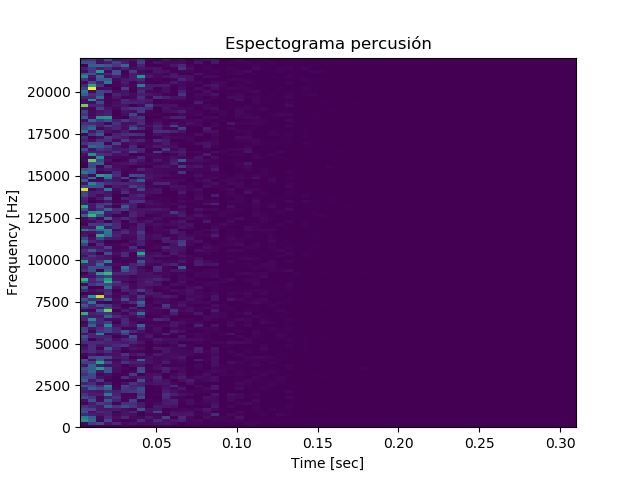
\includegraphics[scale=0.5]{graficos/espectograma_percusion.png}
	\caption{Respuesta en tiempo y en frecuencia de sonido percutido}

	\end{center}
\end{figure}

\subsection{Explicación caja de resonancia}
Se explicará el funcionamiento de la caja de resonancia de una guitarra. No se implementar\'a ya que la necesidad que existe de utilizar dicho elemento en una guitarra es física, en realidad, desde la perspectiva de señales, es posible sintetizar el sonido de una guitarra sin necesidad de simular la caja.
Lo que se busca cuando se fabrica una guitarra es que el sonido generado por el estimo de las cuerdas se propage en una dirección con una intensidad tal, que permita una transmisión efectiva por el aire.
Sin embargo, el aire es un medio de impedancia baja mientras que las cuerdas son una fuente de impedancia alta. Por lo tanto de solo existir las cuerdas el sonido si bien en el sentido más estricto sería producido, no lograría propagarse con intensidad suficiente. 
Por lo tanto surge la necesidad de agregar un elemento f\'isico adicional, la caja de resonancia, que toma el sonido propagado por las cuerdas hacia ``adentro'' y lo vuelve a propagar hacia ``afuera'' con una intensidad mayor, amplificando todas las frecuencias por igual (de lo contrario ocurrir\'ia distorisi\'on). 
\begin{figure}[H]
	\begin{center}
	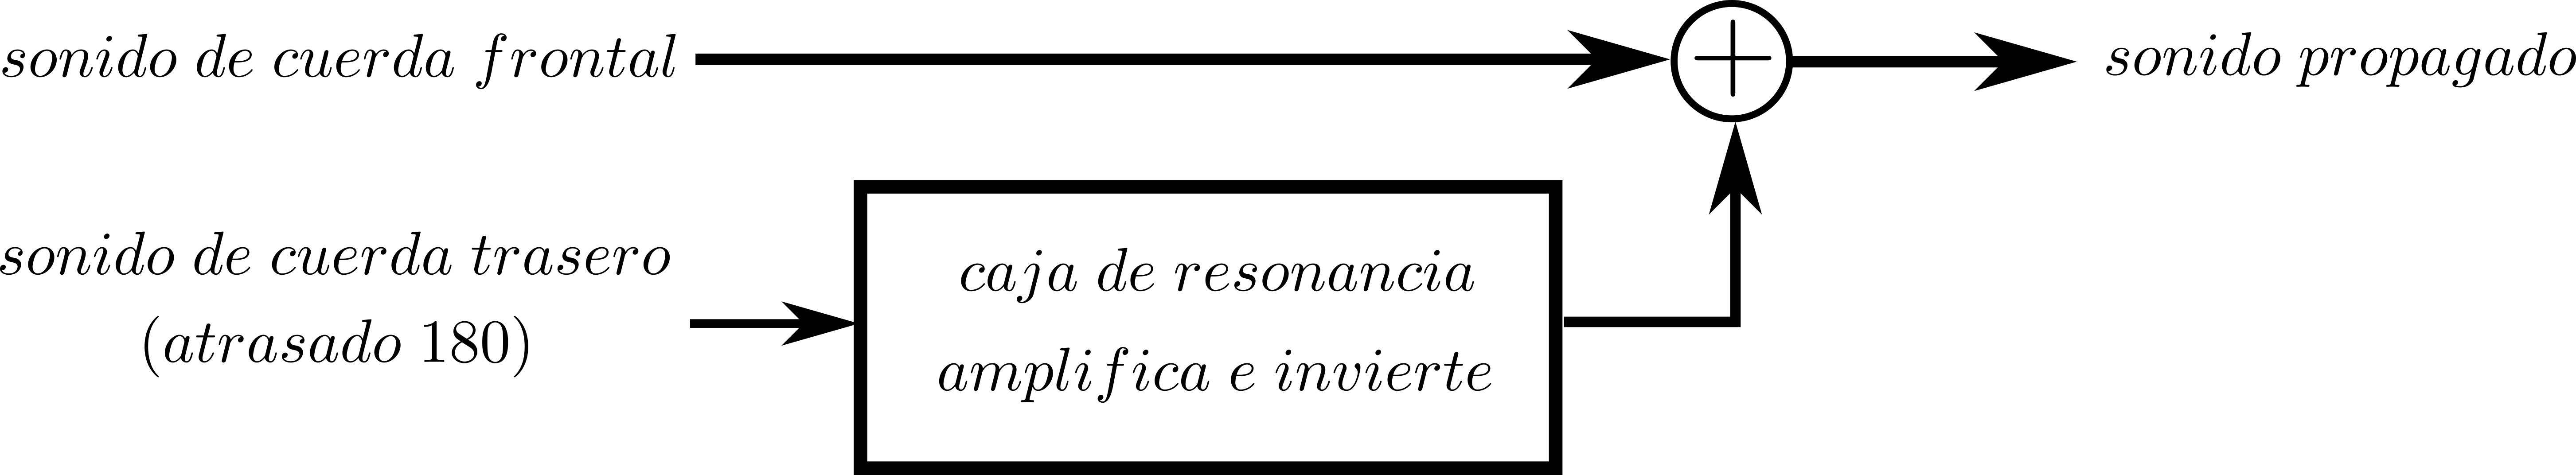
\includegraphics[scale=1.2]{graficos/caja_resonancia.png}
	\caption{Caja de resonancia}

	\end{center}
\end{figure}
Además impone una inversi\'on de fase, idealmente en todas las frecuencias, ya que el sonido propagado por las cuerdas hacia ``adentro'' esta invertido en fase comparando con el emitido por las cuerdas hacia ``afuera''.\par
Los dise\~nos modernos de cajas de resonancia intentan maximizar tanto la inversión de fase como la amplificación de la mayor cantidad de frecuencias, en particular las m\'as bajas que tienen m\'as relevancia en el sonido.


\end{document}